\section{Proposed Method}
\begin{figure}[t]
    \centering
    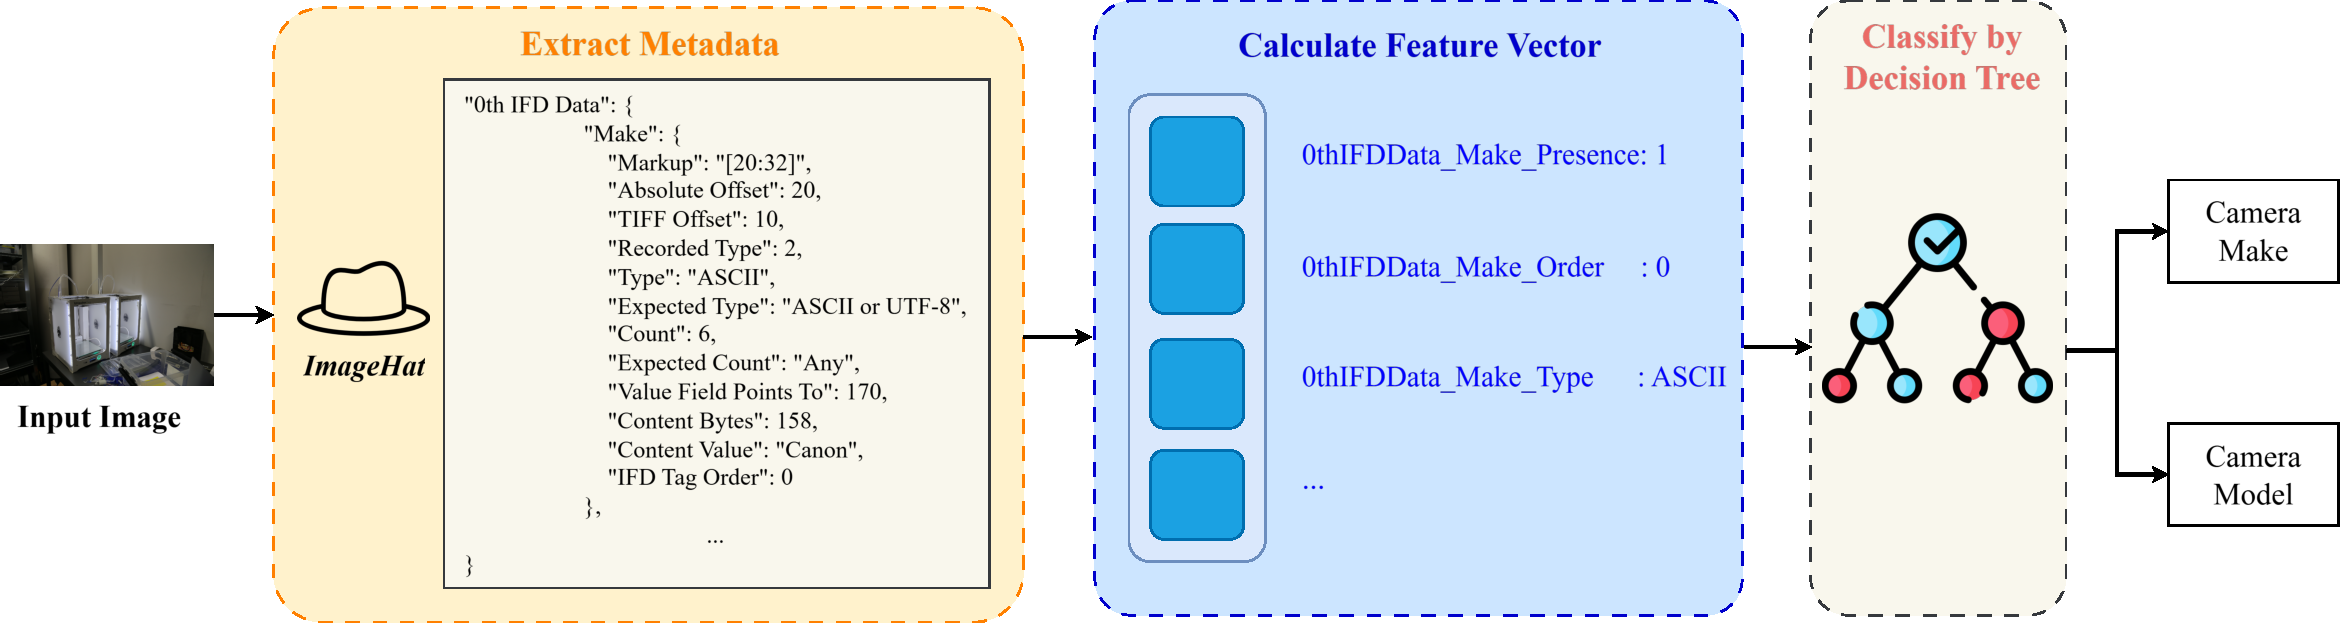
\includegraphics[width=\linewidth]{MMM26'//figures/method.pdf}
    \vspace{-6mm}
    \caption{The proposed method for camera identification.}
    \vspace{-6mm}
    \label{fig:method}
\end{figure}
\subsection{Camera Identification}
Our proposed approach (illustrated in Figure~\ref{fig:method}) utilizes only metadata information from the input image, specifically the presence, order, and type of fields that appear in the Exif file.
Particularly, we deploy ImageHat~\footnote{\url{https://github.com/sinsaegit/ImageHat}}, a powerful Exif reader tool, to obtain the entire structure stored in image data, including file information, JPEG marker segments, Exif header structure, and individual IFD (Image File Directory) entries. Instead of relying on pixel-level characteristics such as sensor pattern noise or CFA traces, we extract metadata descriptors that reflect how a camera model encodes, organizes, and structures its metadata.

To construct feature representations, we parse the metadata and encode the following attributes:
\begin{itemize}
    \item The set of fields present in each dataset is recorded. Then, for every Exif file, each attribute in the block \texttt{BlockName\_FieldName\_Presence} (e.g., \textit{\texttt{0th\_IFD\_\\Data\_Make\_Presence}}, \textit{\texttt{EXIF\_IFD\_Data\_Exposure\_Time\_Presence}}), a value of 1 is assigned if the metadata contains the field inside the block; otherwise, it will be marked as 0.
    \item The attributes within \texttt{BlockName\_FieldName\_Order} receives ordering values within IFD tables.
    \item The attributes within \texttt{BlockName\_FieldName\_Type} receives integer values, which are enumerations of \small \texttt{SHORT}, \texttt{RATIONAL}, \texttt{ASCII}, etc.
\end{itemize}

These features are then transformed into fixed-length vectors, which are used to train standard classifiers (e.g., Decision tree~\cite{decisionTree}, Random decision forest~\cite{ho1995random}). Importantly, since feature names are originally human-readable tags, the model decisions can be interpreted by tracing back predictions to specific entries. This allows forensic investigators to identify which tags or structures are most discriminative for a given camera model.

\begin{figure}[t]
    \centering
    \begin{minipage}{0.48\textwidth}
        \centering
        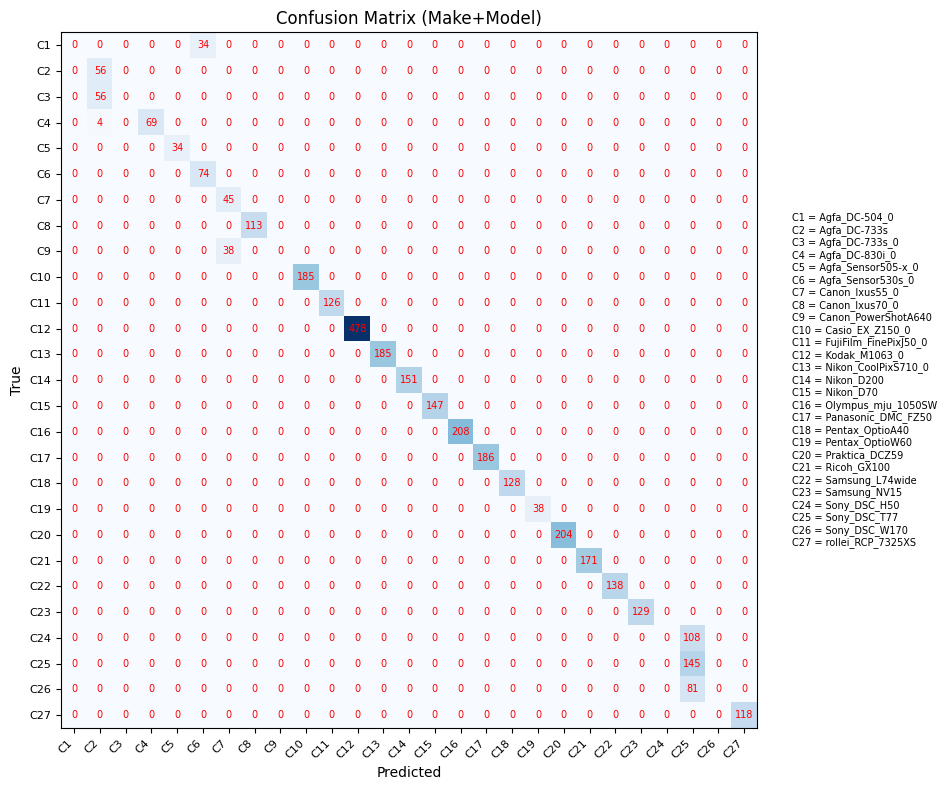
\includegraphics[width=\linewidth]{MMM26'//figures/dresden_make_model_confusion_matrix.png}
        \vspace{-6mm}
        \caption{Confusion matrix of \texttt{Make} and \texttt{Model} classifiers on Dresden dataset~\cite{gloe2010dresden}.}
        \label{fig:dresden_make_model_confusion_matrix}
    \end{minipage} \hfill
    \begin{minipage}{0.48\textwidth}
        \centering
        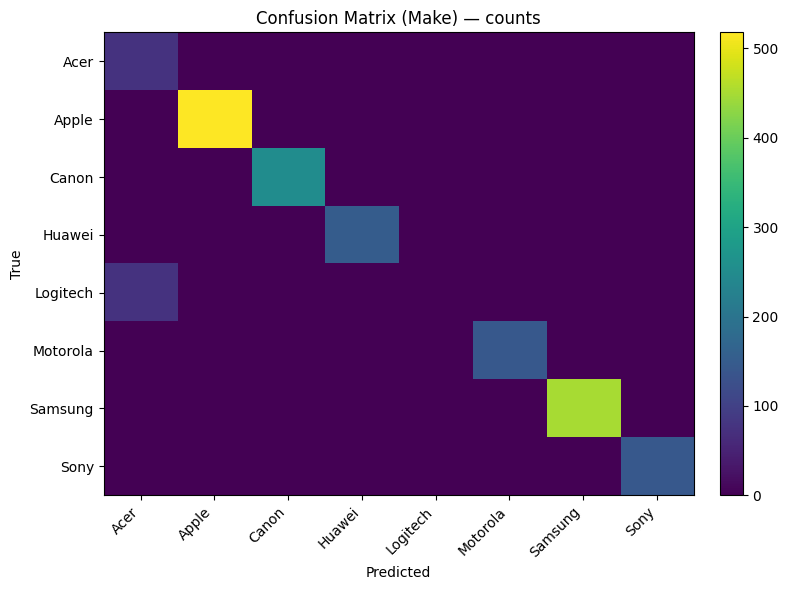
\includegraphics[width=\linewidth]{MMM26'//figures/divnoise_make_random_forest.png}
        \vspace{-6mm}
        \caption{Confusion matrix of camera \texttt{Make} classifiers on DivNoise dataset~\cite{casagrande2023divnoise}.}
        
        \label{fig:divnoise_make_random_forest}
    \end{minipage}    
    \vspace{-3mm}
\end{figure}

\subsection{Metadata Editing Detection}

Our camera identification method performs classification by analyzing the metadata structure, based on the finding that each camera manufacturer and software writes this data in a unique way.
Likewise, metadata editing tools often read and rewrite fields differently from the original software, thereby altering the metadata structure. Hence, we demonstrate this difference by extracting and comparing metadata features in three scenarios: (1) original images versus images with edited metadata using PyExifTool\footnote{\url{https://github.com/smarnach/pyexiftool}}, (2) images before and after being uploaded to and re-downloaded from a social media platform, and (3) images before and after being processed with Adobe Photoshop\footnote{\url{https://www.adobe.com/vn_vi/products/photoshop/online.html}}. In the latter two cases, the Exif data structure may be unintentionally modified.

